%%%%%%%%%%%%%%%%%%%%%%%%%%%%%%%%%%%%%%%%%%%%%%%%%%%%%%%%%%%%%%%%%%%%%%%%%%%%%
%%%
%%% File: thesis.tex, version 1.9, May 2016
%%%
%%% =============================================
%%% This file contains a template that can be used with the package
%%% cs.sty and LaTeX2e to produce a thesis that meets the requirements
%%% of the Computer Science Department from the Technical University of Cluj-Napoca
%%%%%%%%%%%%%%%%%%%%%%%%%%%%%%%%%%%%%%%%%%%%%%%%%%%%%%%%%%%%%%%%%%%%%%%%%%%%%

\documentclass[12pt,a4paper,twoside]{report}         
\usepackage{cs}              
\usepackage{times}
\usepackage{graphicx}
\usepackage{latexsym}
\usepackage{amsmath,amsbsy}
\usepackage{amssymb}
\usepackage[matrix,arrow]{xy}
\usepackage[T1]{fontenc}
\usepackage{ae,aecompl}
%\usepackage{shortcut} %definitii pentru diacritice; 
\usepackage{amstext}
\usepackage{graphics}
\usepackage[T1]{fontenc}
\usepackage{ae,aecompl}
\usepackage{algorithm}
%\usepackage{algorithmic}
\usepackage{color}
\usepackage{color}
\usepackage[super]{nth}
% \mastersthesis
\diplomathesis
% \leftchapter
\centerchapter
% \rightchapter
\singlespace
% \oneandhalfspace
% \doublespace

\renewcommand{\thesisauthor}{Mihai PÎȚU}    %% Your name.
\renewcommand{\thesismonth}{September}     %% Your month of graduation.
\renewcommand{\thesisyear}{2019}      %% Your year of graduation.
\renewcommand{\thesistitle}{SueC - An Editor and Interpreter for Pseudocode} 
\renewcommand{\thesissupervisor}{dr. eng. Emil Ștefan CHIFU}
\newcommand{\department}{\bf FACULTY OF AUTOMATION AND COMPUTER SCIENCE\\
COMPUTER SCIENCE DEPARTMENT}
\newcommand{\thesis}{LUCRARE DE LICEN'T'A}
\newcommand{\utcnlogo}{
\includegraphics[width=15cm]{img/tucn.jpg}}

\newcommand{\uline}[1]{\rule[0pt]{#1}{0.4pt}}
%\renewcommand{\thesisdedication}{P\u{a}rin\c{t}ilor mei}

\begin{document}
%\frontmatter
%\pagestyle{headings}

\newenvironment{definition}[1][Defini\c{t}ie.]{\begin{trivlist}
\item[\hskip \labelsep {\bfseries #1}]}{\end{trivlist}}



%\thesistitle                    %% Generate the title page.
%\authordeclarationpage                %% Generate the declaration page.

\pagenumbering{arabic}
\setcounter{page}{4}



\begin{center}
\utcnlogo

\department

\vspace{4cm}

{\bf \thesistitle} %LICENSE THESIS TITLE}

\vspace{1.5cm}

LICENSE THESIS

\vspace{6cm}

Graduate: {\bf \thesisauthor} 

Supervisor: {\bf \thesissupervisor}

\vspace{3cm}
{\bf \thesisyear}
\end{center}

\thispagestyle{empty}
\newpage

\begin{center}
\utcnlogo

\department

\end{center}
\vspace{0.5cm}

%\begin{small}
\begin{tabular}{p{7cm}p{8cm}}
 %\hspace{-1cm}& APPROVED,\\
 \hspace{-1cm}DEAN, & HEAD OF DEPARTMENT,\\
 \hspace{-1cm}{\bf Prof. dr. eng. Liviu MICLEA} & {\bf Prof. dr. eng. Rodica POTOLEA}\\  
\end{tabular}
 
\vspace{2cm}

\begin{center}
Graduate: {\bf \thesisauthor}

\vspace{1cm}

{\bf \thesistitle}
\end{center}

\vspace{1cm}

\begin{enumerate}
 \item {\bf Project proposal:} {\it Short description of the license thesis and initial data}
\item {\bf Project contents:} {\it (enumerate the main component parts) Presentation page, advisor's evaluation, title of chapter 1, title of chapter 2, ..., title of chapter n, bibliography, appendices.}
\item {\bf Place of documentation:} {\it Example}: Technical University of Cluj-Napoca, Computer Science Department
\item {\bf Consultants:}
\item {\bf Date of issue of the proposal:} November 1, 2017
\item {\bf Date of  delivery:} February 18, 2019 {\it (the date when the document is submitted)}
  \end{enumerate}
\vspace{1.2cm}

\hspace{6cm} Graduate: \uline{6cm} 

\vspace{0.5cm}
\hspace{6cm} Supervisor: \uline{6cm} 
%\end{small}

\thispagestyle{empty}


\newpage
$ $
%\begin{center}
%\utcnlogo

%\department
%\end{center}

\thispagestyle{empty}
\newpage

\begin{center}
\utcnlogo

\department
\end{center}

\vspace{0.5cm}

\begin{center}
{\bf
Declara\c{t}ie pe proprie r\u{a}spundere privind\\ 
autenticitatea lucr\u{a}rii de licen\c{t}\u{a}}
\end{center}
\vspace{1cm}



Subsemnatul(a) \\
\uline{14.8cm}, 
legitimat(\u{a}) cu \uline{4cm} seria \uline{3cm} nr. \uline{4cm}\\
CNP \uline{9cm}, autorul lucr\u{a}rii \uline{2.8cm}\\
\uline{16cm}\\
\uline{16cm}\\
elaborat\u{a} \^{\i}n vederea sus\c{t}inerii examenului de finalizare a studiilor de licen\c{t}\u{a} la Facultatea de Automatic\u{a} \c{s}i Calculatoare, Specializarea \uline{7cm} din cadrul Universit\u{a}\c{t}ii Tehnice din Cluj-Napoca, sesiunea \uline{4cm} a anului universitar \uline{3cm}, declar pe proprie r\u{a}spundere, c\u{a} aceast\u{a} lucrare este rezultatul propriei activit\u{a}\c{t}i intelectuale, pe baza cercet\u{a}rilor mele \c{s}i pe baza informa\c{t}iilor ob\c{t}inute din surse care au fost citate, \^{\i}n textul lucr\u{a}rii \c{s}i \^{\i}n bibliografie.

Declar, c\u{a} aceast\u{a} lucrare nu con\c{t}ine por\c{t}iuni plagiate, iar sursele bibliografice au fost folosite cu 
respectarea legisla\c{t}iei rom\^{a}ne \c{s}i a conven\c{t}iilor interna\c{t}ionale privind drepturile de autor.

Declar, de asemenea, c\u{a} aceast\u{a} lucrare nu a mai fost prezentat\u{a} \^{\i}n fa\c{t}a unei alte comisii de examen de licen\c{t}\u{a}.

\^{I}n cazul constat\u{a}rii ulterioare a unor declara\c{t}ii false, voi suporta sanc\c{t}iunile administrative, respectiv, \emph{anularea examenului de licen\c{t}\u{a}}.

\vspace{1.5cm}

Data \hspace{8cm} Nume, Prenume

\vspace{0.5cm}

\uline{3cm} \hspace{5cm} \uline{5cm}

\vspace{0.5cm}
\hspace{9.4cm}Semn\u{a}tura

\thispagestyle{empty}

\newpage


%\listoftables
%\listoffigures

%\clearpage 
%\newpage

%\begin{comment}
{\color{red}{\bf De citit \^{\i}nainte} (aceast\u{a} pagin\u{a} se va elimina din versiunea final\u{a})}:
\begin{enumerate}
 \item Cele trei pagini anterioare (foaie de cap\u{a}t, foaie sumar, declara\c{t}ie) se vor lista pe foi separate (nu fa\c{t}\u{a}-verso), fiind incluse \^{\i}n lucrarea listat\u{a}. 
 Foaia de sumar (a doua) necesit\u{a} semn\u{a}tura absolventului, respectiv a coordonatorului.
 Pe declara\c{t}ie se trece data c\^{a}nd se pred\u{a} lucrarea la secretarii de comisie.
 \item Pe foaia de cap\u{a}t, se va trece corect titulatura cadrului didactic \^{\i}ndrum\u{a}tor, \^{\i}n englez\u{a} (consulta\c{t}i pagina de unde a\c{t}i desc\u{a}rcat acest document pentru lista cadrelor didactice cu titulaturile lor).
 \item Documentul curent {\bf nu} a fost creat \^{\i}n MS Office. E posibil sa fie mici diferen\c{t}e de formatare. 
\item Cuprinsul \^{\i}ncepe pe pagina nou\u{a}, impar\u{a} (dac\u{a} se face listare fa\c{t}\u{a}-verso), prima pagin\u{a} din capitolul \emph{Introducere} tot a\c{s}a, fiind numerotat\u{a} cu 1. % Pentru actualizarea cuprinsului, click dreapta pe cuprins (zona cuprinsului va apare cu gri), Update field-$>$Update entire table.
\item E recomandat s\u{a} vizualiza\c{t}i acest document \c{s}i \^{\i}n timpul edit\u{a}rii lucr\u{a}rii. % după ce activaţi vizualizarea simbolurilor ascunse de formatare (apăsaţi simbolul  din Home/Paragraph).
\item Fiecare capitol \^{\i}ncepe pe pagin\u{a} nou\u{a}. % datorită simbolului ascuns Section Break (Next Page) care este deja introdus la capitolul precedent. Dacă ştergeţi din greşeală simbolul, se reintroduce (Page Layout -> Breaks).
\item Folosi\c{t}i stilurile predefinite (Headings, Figure, Table, Normal, etc.)
\item Marginile la pagini nu se modific\u{a}.
\item Respecta\c{t}i restul instruc\c{t}iunilor din fiecare capitol.
\end{enumerate}
 
%\end{comment}

\newpage

\tableofcontents
\newpage

\chapter{Introduction - Project Context}
\pagestyle{headings}
\section{Project Context}

	Computer science and programming is taught in schools around Romania for at least 30 years, especially in high schools, but also in secondary schools, starting with the \nth{5} grade. Before introducing directly to a programming language, many teachers use a pseudocode language which serves as a mean of understanding programming concepts in a more universal manner, bringing it closer to the natural spoken language. I have decided to make an implementation of this pseudocode by creating an editor and interpreter for it.
	
	The purpose of this project is to create an easier way of learning programming concepts for students who are new into this domain. This will serve as a fresh renewal of software used in schools today, as older tools such as Code::Blocks and/or Free Pascal are still used in schools and programming contests.
 
	SueC is the name of the editor which creates, edits and compiles files which represent pseudocode files. This editor will work also like any other editors, providing some error-checking mechanisms and returning the result after compiling a pseudocode file.
	
\section{Motivation}
	During high school, many of my colleagues have struggled learning programming and computer science as they had issues in understanding the simple paradigms because of C programming language. They have improved throughout the high school due to the teacher using pseudocode as a mean of explaining simple algorithms and paradigms, but there were some struggle shown for some when changing the pseudocode into implementations in C. 
	
	Nowadays, this issue is still persistent in schools in Romania as C and Pascal are used as main programming languages for teaching, exams and computer science contests. There are some more interactive programming languages such as Scratch which uses a graphical interface for implementing simple programs, but since the target audience is for primary school students, there is a need for an attractive way of making secondary and high school students for understanding programming at their age group. 
	
	At the moment, there are platforms for learning code such as CodeCademy and Udemy which contain basic courses for people at every age, but the main focus is for people who have a little background in programming and computer science.
	
	

\chapter{Project Objectives and Specifications}


As the title of the project suggests - "An Editor and Interpreter for Pseudocode" - this is an application which will serve as an educational tool for using the pseudocode as a programming language.

For the users of this application(students and/or teachers), the main functionalities of this application are:
\begin{itemize}
	\item Creating/opened a file in which pseudocode can be implemented.
	\item Writing pseudocode in the file created/opened.
	\item Compiling the file and obtaining the desired result or error(s) if there are occured.
	\item Running some step-by-step basic tutorials which are aimed for learning the language.
\end{itemize}


The main objectives of this project are:
\begin{itemize}
	\item Developing an user-friendly application which handles the main file handling operations and communicating with the compiler of the pseudocode source files.
	\item Creating an understandable programming language that resembles the pseudocode used by teachers in schools and/or universities. For a technical point of view, the pseudocode will be created like any other programming languages, having similar elements to existing ones that are used nowadays, but also with specific structural elements bringing it closer to the natural language.
	\item Developing a compiler for this programming language by defining a lexical and syntactic analyzer respectively. These analyzers contain the set of rules that apply to the programming language. 
\end{itemize}





\chapter{Bibliographic research}

For this project, my research done was focused on the main components and technologies included in the project:
\begin{enumerate}\bfseries
	\item C Programming Language
	\item Python Programming Language
	\item Lex
	\item Yacc
\end{enumerate}
 
\section{C Programming Language}
 C is a general-purpose, procedural computer programming language supporting structured programming, lexical variable scope, and recursion, while a static type system prevents unintended operations. This programming language was created between 1972 and 1973 as a way of making utilities work in Unix operating system, later being used for reimplementing the kernel of this OS. Since 1980s, C has gained enough popularity becoming one of the most widely used programming languages in the world. During this time, there were several C compilers created by several vendors for being available for the majority of existing computer architectures and operating systems. Since 1989, C has been standardized by ANSI (American National Standards Institute) and by the International Organization for Standardization (ISO). 
  
 Being an imperative procedural language, C was designed to be compiled using a relatively straightforward compiler to provide low-level access to memory and language constructs that map efficiently to machine code instructios all with minimal runtime support. This language supports cross-platform programming, making it available in numerous platforms, from embedded microcontrollers and supercomputers. It also stood as a big influence in the creation of other programming languages, such as:
 \begin{itemize}
 	\item C++
 	\item C\#
 	\item Java
 	\item Python
 	\item Go
 \end{itemize}

 The C programming language syntax is defined by a formal grammar, having specific keywords and rules based on statements to specify different actions. The most common statement is an expression statement, consisting of an expression to be evaluated followed by a semicolon. The main structure of a C program consists of declarations and function definitions, which in turn contain declarations and statements. 
 
 Besides exxpressions, the main sequence execution of statements can contain several control-flow statements defined by reserved keywords:
  
 \begin{itemize}
 	\item Conditional execution 
 	
 		This is defined by \textit{if} and \textit{else} statements. These statements contain an expression that the \textit{if} checks if it is true or not and execute statements based on a condition.
 		
 		Alongside those statements, there exists the \textit{switch} statement in which it displays a \textit{case} based on the expression given.
 		
 	\item Iterative execution (Looping)
 	
 		This is defined by \textit{while} , \textit{do-while} and \textit{for} statements which can loop through a certain set. The \textit{for} statement contains separate expressions for initialization, testing and reinitialization, any of which can be omitted. 
 \end{itemize}


\section{Python Programming Language}

Python is an interpreted, high-level, general-purpose programming language with the aim to help programmers with clear, logical code for small and large-scale projects. It was conceived in the late 1980s as a successor to ABC language, but it was released in 1991. Python is dynamically typed and garbage-collected, supporting multiple programming paradigms, such as: procedural, object-oriented and functional. Due to this and its comprehensive standard library, Python is often described as a "batteries included" language. 

Due to supporting multiple programming paradigms, Python is used in a lot of domains. Object-oriented programming and structured programming are fully supported, but it also includes features from functional programming and aspect-oriented programming. Other paradigms can be supported by Python via extensions, including even logic programming and design by contract. 

Python is meant to be an easily readable language due to its syntax and semantics. The format is visually uncluttered, using English keywords more often than punctuation. Curly brackets are not used to delimit blocks and semicolons are optional. For block delimitation, whitespace indentation is used. A decrease in indentation shows that the current block of code is finished. With this method, it is shown that the program's visual structure accurately represents the program's semantic structure. 

\section{Technologies used}

\subsection{Lex}

Lex is a computer program designed for generating lexical analyzers. It is the standard lexical analyzer generator on many Unix systems, having an equivalent tool as part of the POSIX standard. It is commonly used with \textit{yacc} parser generator.

Lex reads an input stream specifying the lexical analyzer and outputs source code implementing a lexer in C. This input stream is given to Lex directly as standard input from the user or a file that contains the 

\subsection{Yacc}

Yacc\textit{(Yet Another Compiler-Compiler)} is a computer program for the Unix operating system. It is a LALR\textit{(Look Ahead Left-to-Right)} parser generator, which generates a parser, the part of a compiler that tries to make syntactic sense of the source code. 

\subsection{Java Programming Language}
Java is a general-purpose programming language that is object-oriented and class-based. It is designed to have as few implementation dependencies as possible, with the intention to letting application developers apply the WORA rule (Write Once, Run Anywhere) - all compiled Java code can run on all platforms that support Java without the need for recompilation. 
Java applications are typically compiled to bytecode that can be run on any Java Virtual Machine (JVM), regardless of the underlying computer and/or software architecture. 

This programming language has been designed in May 1995 by James Gosling from Sun Microsystems (now being acquired by Oracle) being licensed under the same companu. Since May 2007, Java has been relicensed under GNU General Public License with the original Java compilers, virtual machines and class libraries. Nowadays, this programming language is one of the most popular programming languages in use, mainly for client-server applications. 

The syntax of Java is similar to C and C++, but it has fewer low-level facilities than either of them. The main draw for the programming language is being class-based. Classes are a code template for creating objects, providing initial values for state (variables/attributes) and implementations of behavior (methods). Besides creating objects, a class can be used as a standalone program, running imperatively as any C or C++ program. The main goals in the creation of this language are:
\begin{itemize}
 \item The language must be simple, object-oriented and familiar.
 \item The language must be robust and secure.
 \item The language must be architecture-neutral and portable.
 \item The language must execute with high performance.
 \item The language must be interpreted, threaded and dynamic.
\end{itemize}


\subsection{Java Swing UI}

Java Swing is a GUI widget toolkit for Java, creating desktop applications similar to Windows Forms. It provides a more sophisticated set of GUI components than the earlier Abstract Window Toolkit (AWT), making it easir to emulate application functionalities with powerful and flexible components. 

This framework follows a single-threaded programming model, applying functionalities similar to Model-View-Controller design pattern. Each Swing component has an associated model specified in terms of a Java interface that can be used either as the default implementation or as a variation of the component created by the developer. Based on this model and the MVC pattern, it offers loose coupling between components and elements of the application.


\chapter{Analysis and Theoretical Foundation}
\section{Editor Application}
\subsection{Model-View-Controller(MVC) Architecture}

Model-View-Controller (MVC) is a software design pattern commonly used for developing user interfaces which divides the related program logic into three interconnected elements. It is used mainly for designing the layout of a page (Desktop or Web). Although it has been traditionally used for desktop applications, this pattern has become popular in designing web applications. There are specified MVC frameworks for web and mobile application development in popular programming languages like: Java, C\#, Swift, Python, Ruby, JavaScript and PHP.


The main components of this design pattern are:

\begin{itemize}
\item \textbf{Model}
		
It represents the central component of the pattern, being the application's dynamic data structure, independent of the user interface. It directly manages the data, logic and rules of the application.

\item \textbf{View}

It represents the visual element of the pattern, being any representation of information possible, like: charts, tables, diagrams, pages, forms etc. 

\item \textbf{Controller}

Accepts input from the view and converts the data obtained into commands that are directed to the model and/or view.
\end{itemize}

\begin{figure}
	\centering
	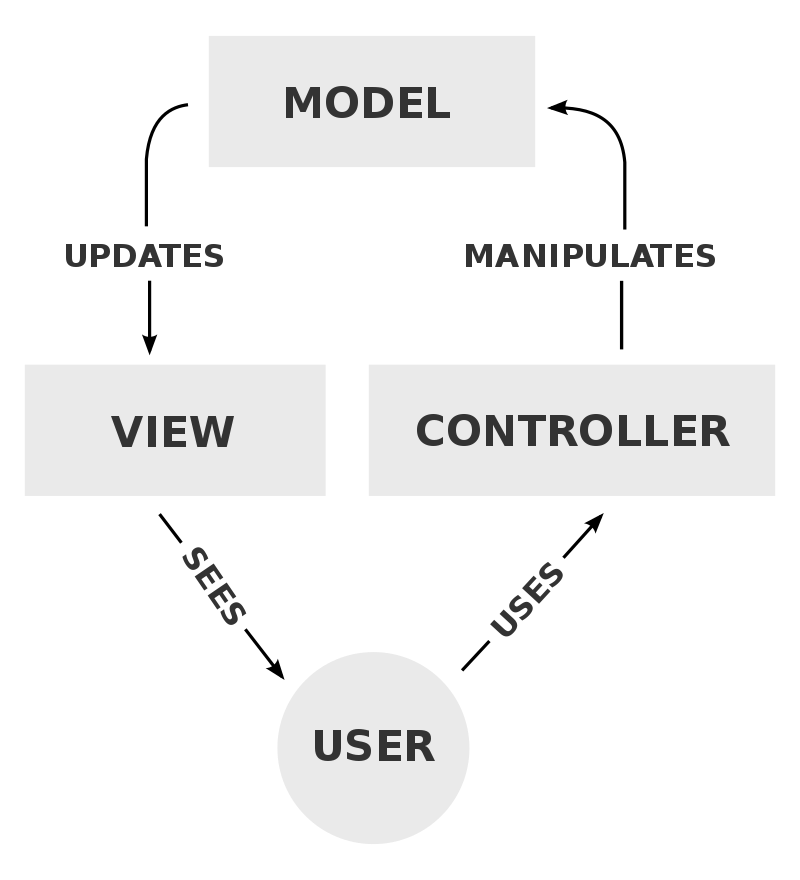
\includegraphics[scale=0.2]{img/MVCDiag.png}
	\caption{Model-View-Controller Diagram}
\end{figure}

Besides the division of the application into these components, this pattern defines the interactions between the components:

\begin{itemize}
	\item The model of the application is responsible for managing the data of the application. The user input is received from the controller.
	\item The view represents a presentation of the model having a particular format.
	\item The controller responds to the user input given in the view(s) and performs interactions on the data model objects.
\end{itemize}

Model-View-Controller pattern offers different advantages in regards to developing applications, such as:
\begin{itemize}
	\item \textbf{Simultaneous development over the code} 
	
	Multiple developers can work simultaneously on the model, controller and views, having no change in the actual structure of the system.
	\item \textbf{High cohesion}
			
	The cohesion is defined in computer programming as the degree to which the elements inside a module belong together. In other terms, it acts as a measure of the strength of relationship between the methods and data of one class and some unifying purpose or concept served by the class.
	
	In object-oriented programming, the term "cohesion" is used quite frequently together with coupling. The methods that serve in a class tend to be similar in many aspects, then that class is said to have high cohesion. A highly cohesive system has a manageable complexity, due to the increase of code readability and reusability. 
	
	This pattern presents this characteristic by having logical groupings of related actions in one controller altogether. Also, multiple views that are associated to a model can be grouped together. 
	
	\item \textbf{Loose coupling}
	
	Besides the cohesion, which serves the degree of "togetherness" of elements inside a module, the coupling is described as the degree of independence between software modules i.e. the strength of the relationships between modules between a system.
	
	A loosely coupled system is one which each of its components makes use of little or no knowledge of the definitions of other separated components. The main subareas include the coupling of classes, interfaces, data and services. Loose coupling goes hand-in-hand with high cohesion by having an manageable complexity and the ease of use of alternative implementations that provide the same services. 
	
	In the case of Model-View-Controller pattern, its nature and workflow shows the existence of a loose coupling between the Model, View and Controller of the application.	

\end{itemize} 

	
\section{Interpreter}

An interpreter is a computer program that directly executes instructions written in a programming or scripting language, without requiring them to have been compiled into a machine code language program. For program execution, an interpreter uses one of these strategies:

\begin{itemize}
	\item Parsing the source code and performing its behavior directly;
	\item Translating the source code into efficient intermediate representation and immediately execute this;
	\item Explicitly execute stored precompiled code made by a compiler which is part of the interpreter system.
\end{itemize}

Historically speaking, interpreters have been used since 1952 to ease programming within the limitations of computers existing at that time. Another usage of them was to translate between low-level machine languages, allowing code to be written for machines that were still under development and tested on computers that already existed. The first interpreted high-level language was Lisp. Nowadays, programs written in a high-level language are either directly executed by some kind of interpreter or converted into machine code by a compiler for the CPU to execute.

There are some differences between a compiler and interpreter, mainly in the functionality. A compiler works most of the time with an assembler and linker. It produces machine code most of the time to be executed by the computer hardware, but it can often produce object code, an intermediate form. An object code is the same machine code created before, but with the addition of a symbol table containing names and tags to make executable blocks (or modules) identifiable and relocatable. The linker comes into working by combining these object file(s) with libraries that are included in the compiler in order to create a single executable file. On the other hand, a interpreter written in a low-level language may have similar machine code blocks implementing functions of the high level language stored and executed when a function's entry in a look up table points to that code. However, an interpreter written in a high level language uses another approach, such as: generating and walking a parse tree, generating and executing intermediate software-defined instructions or both approaches.

Both compilers and interpreters generally turn source code into tokens, generate a parse tree. The basic difference is that a compiler system (along with a linker) generates a stand-alone machine code program, whereas an interpreter system performs the actions described by the high level program.

For this project, this interpreter is written in C, a high level language, being split into three parts:
\subsection{Lexical Analyzer}
	
	Lexical analysis (or tokenization) is the process of converting a sequence of characters into a sequence of tokens. A program that performs lexical analysis is called a lexer or tokenizer.
	
	In modern processing, a lexer forms the first phase of a compiler frontend, occuring mostly in one pass of the source code. A lexer is used alongside with a parser in most compilers and interpreters. It splits the source code, sentence by sentence, into tokens. Tokens are strings with an assigned meaning, being structured as a pair consisting of a token name and an optional token value. The token names can generally be split into:
	
	\begin{itemize}
		\item \textit{Identifiers} - Names that a programmer/developer chooses.
		\item \textit{Keywords} - Names that are already defined in the programming language
		\item \textit{Separators/Punctuators} - Punctuation characters and paired-delimiters
		\item \textit{Operators} - Symbols that operate on arguments and produce results
		\item \textit{Literals} - Numeric, logical, textual, reference literals
		\item \textit{Comments} - Line, block comments 
	\end{itemize}
	
	When a statement is given as a source, the lexer splits every element of the statement, creating one token per element. For example, we consider a C expression: 
	
	\textit{c = a * (b + 5);}
	
	The lexer gets this statement, passes through its all defined lexems (the source program that matches the pattern for a token) and creates the token based on their lexem appartenance. In this case, the statement is split into tokens that are categorised:
	\begin{table}[H]
	\centering
\begin{tabular}{|c|c|c|c|l}
\cline{1-4}
\multicolumn{1}{|l|}{identifier} & \multicolumn{1}{l|}{operator} & \multicolumn{1}{l|}{separator} & \multicolumn{1}{l|}{literal} &  \\ \cline{1-4}
c                                & =                             & (                              & 5                            &  \\ \cline{1-4}
a                                & *                             & )                              &                              &  \\ \cline{1-4}
b                                & +                             & ;                              &                              &  \\ \cline{1-4}
\end{tabular}
\end{table}

	The tokens obtained are, then, passed to the parser.
	
\subsection{Syntactic Analyzer}
	Syntactic analysis (or parsing) is the process of analyzing a string of symbols, either in natural language, computer languages or data structures, conforming to the rules of a formal grammar. In computer science, a parser is a software component that takes input data and builds a data structure - often a parse tree, abstract syntax tree or other hierarchical structure, giving a structural representation of the input while checking for correct syntax. In most cases, a lexer works hand-in-hand with a parser.
	
	After obtaining the tokens from the lexer, each token is analyzed based on its token name and creates a parse tree which is needed for passing through in order to get an order of operation handling, giving the response. 
	%\ Aci bag exemplul cu diagrama pe care o folosesc si la parse tree si explic de frunze ca-s identificatori/literali
\subsection{Parse Tree}
 	
 	The parse tree is the result of parsing the tokens from the lexer. Passing the tree determines the order of the operations done, giving the results. There are two ways of performing the pass of the tree:
 	
 	\begin{itemize}
 		\item \textbf{Top-down parsing}
 		
 		This method can be viewed as an attempt to find the left-most derivations of an input stream by searching for parse trees using a top-down expansion of the given formal grammar rules. Tokens are consumed from left to right.
 		
 		\item \textbf{Bottom-up parsing}
 		
 		A parser can start with the input and attempt to rewrite it to the start symbol. In this case, the input is represented by the leaves of the parse tree, being the most basic elements. The best example of this case are the LR(Left-to-right Rightmost) parsers, which analyze deterministic context-free languages in linear time.
 	\end{itemize}

\chapter{Detailed Design and Implementation}

\section{Project Component Diagram}
\begin{figure}[h]
 \centering
 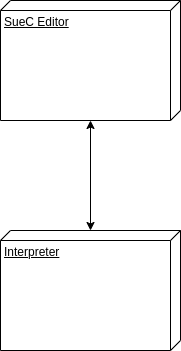
\includegraphics[scale=0.6]{img/CompDiag.png}
 \caption{Component Diagram}
\end{figure}

This project is split into two main components:
\begin{itemize}
	\item Editor Application
	\item SueC Interpreter
\end{itemize}

These components communicate bidirectionally in order to ensure a good workflow:
\begin{itemize}
	\item The editor application runs the interpreter that compiles the source file via running the Linux process.
	\item The result from the interpretation is then written in a file that is read by the editor application and displayed it there.  
\end{itemize}


\section{Editor Application}
The editor application is a Java Swing Desktop application that acts as the main interface of compiling SueC code files. The main purpose of creating it was to have a simple and easy-to-read graphical user interface for an user to create, edit and run SueC code files.
\subsection{Packages}

The main structure of the application (see Figure 5.2) is based on the Model-View-Controller pattern:
\begin{itemize}
 \item The \textit{Model} component is represented by the main models used in the project.
 \item The \textit{View} component is represented by the Swing views created to display specific tasks.
 \item The \textit{Controller} component is already integrated into the Java Swing architecture, as these are represented by the event handlers used for each component used in each view.
\end{itemize}

\begin{figure}[h]
 \centering
 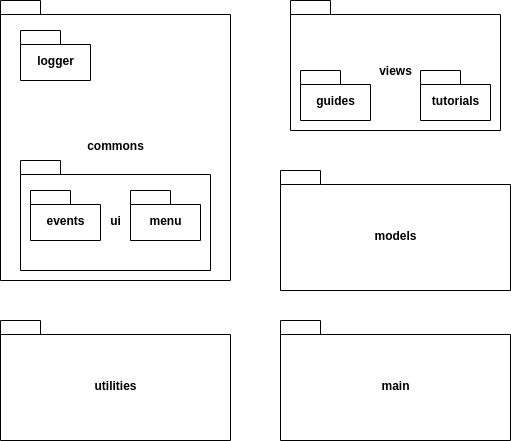
\includegraphics[scale=0.5]{img/packagediag.png}
 \caption{Package Diagram}
\end{figure}

Besides the MVC-like packages, there are also packages used for other functionalities that are used to ensure the workflow of the Editor App and the SueC Interpreter.

\begin{enumerate}
 \item \textbf{\textit{models} package}
 
 \begin{figure}[h]
 \centering
 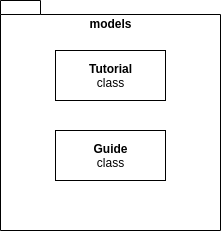
\includegraphics[scale=0.4]{img/ModelsPackage.png}
 \caption{Class diagram of \textit{models} package}
\end{figure}

This package contains the main models used in the project for representing the educational part of the application.  
\begin{itemize}
 \item \textbf{Tutorial} class
    
    This class resembles a simple version of a tutorial object. It is used for adding the tutorial data for the tutorial views. Each tutorial contains:
    \begin{itemize}
        \item \textit{id} - the number associated to the tutorial
        \item \textit{title} - the title of the tutorial
        \item \textit{description} - the description of the tutorial
        \item \textit{task} - the task required for the user to finish the tutorial
        \item \textit{answer} - the expected answer that the interpreter should give after the user runs the task.
    \end{itemize}
    
    \item \textbf{Guide} class
    
    This class resembles a simple version of a guide object. It is used for adding the guide data for the guide views. Each tutorial contains:
    \begin{itemize}
        \item \textit{id} - the number associated to the guide
        \item \textit{title} - the title of the guide
        \item \textit{description} - the description of the guide
        \item \textit{example} - am example of usage of the notion described in the guide
    \end{itemize}
\end{itemize}
These resource files are JSON files - \textit{tutorials.json} and \textit{guides.json} - that contain a list of tutorial and guide objects, respectively. The lists are then used for displaying the tutorials/guides in the application. The model classes are used as the template objects for these JSON resource files.

\item \textbf{\textit{views} package}

\begin{figure}[H]
    \centering
    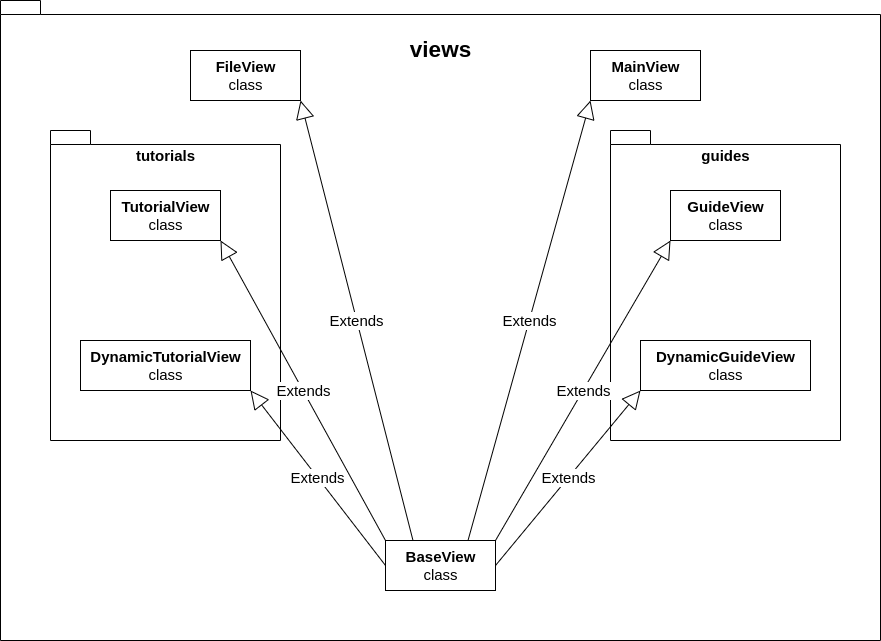
\includegraphics[width=0.8\linewidth]{img/ViewsPackage.png}
    \caption{Views Package}
    \label{fig:conf}
\end{figure}

This package contains all the view classes that are displayed in the application. These classes have been made using components from Java Swing that were directly used or extended in objects from the \textbf{\textit{commons}} package.

All views that are shown are created from extending the \textbf {BaseView} class. This class holds the main structure of the views, all other views being extended from this. Itself, it is extended from \textbf{JFrame} class that comes from Swing library - creating the actual frame that is displayed to the user. The view consists of:
\begin{itemize}
 \item \textbf{Main Menu Bar} - it is defined in the \textbf{\textit{commons}} package as a \textbf{MainMenuBar} object, an extension of the associated Swing object. It holds all of the menus that are also defined and used throughout the views. 
 \item \textbf{Help Menu} - one of the defined menus created  in \textbf{\textit{commons}} package and used in all the views. It is a \textbf{HelpMenu} object. 
 \item \textbf{Main Panel} - a JPanel object that serves as the main panel of the JFrame. Each view adds elements only to this element, as it is structured as a grid with one column and two or three columns, depending on the view.
\end{itemize}

The other views are created and grouped based on their functionality. These views are linked via events that are triggered by accessing the menu options from the menu bar.  

\begin{enumerate}
 \item \textbf{Main View - MainView} class
 
 This view is the first view that can be seen when running the application. It is used as a welcome screen at the start of the application. The main panel contains only two labels that display a welcome message to the app.
 
 \item \textbf{File View - FileView} class
 
 This view represents the editor where an user can edit and compile SueC source code. It can be accessed when creating or opening a SueC source code file. The main panel contains two text areas:
 \begin {itemize}
  \item \textbf{Code text area}
  
  This area is used by the user to write the source code. At the start of the view lifecycle, this text area is loaded with the contents of the source file. After that, the user can edit the contents of the source code using that text area and save it or compile the code.
  
 \item \textbf{Output text area}
 
 This area is used by the user to see the output after compiling the code written in the code area. This area is read-only and it can only be modified by the output of the compiler. 
 \end {itemize}

 The design of the view is quite simple as it holds a straightforward approach towards using the application. The user can write the code in the code text area, run the compiler by accessing the compile menu and pressing "Compile file...". Then, the output is shown in the output text area. 
 
 \item \textbf{Tutorial View - TutorialView}
 
 This view is the main menu view for the tutorials. It holds the structure of \textbf{BaseView}, but the main panel layout being a three-rows grid. The first two rows hold a welcome message for getting into the menu. The last row is split in two columns.
 \begin{itemize}
  \item The left column contains a button with label \textit{Start Tutorials}. When pressing the button, the user is redirected to the first tutorial of the tutorial list.
  \item The right column is a JList that contains the tutorials that are loaded at the start of the application life cycle. When pressing on one tutorial from the list, the user is redirected to that specified tutorial and starts the tutorials from that selected item. 
 \end{itemize}
 
 After running all the tutorials, the user is redirected back to this view.
 
 \item \textbf{Dynamic Tutorial View - DynamicTutorialView}
 
 This view represents the actual tutorial structure and has the tutorial elements implemented. Structurally, the main panel is 
 also split into three rows:
 \begin{itemize}
 \item \textbf{Top Panel}
 
 This panel serves as a command panel. It is split into three columns and contains:
 \begin{itemize}
    \item \textit{Back} button 
        
        It redirects the user to the previous tutorial. This button is not shown in the first tutorial.
    \item Title label 
        
        A label that contains the title of the tutorial.
    \item \textit{Next/Finish} button
    
        Excepting the last tutorial, the button displayed is a \textit{Next} button that, when clicked, the user is redirected to the next tutorial. 
        
        At the last tutorial, when finished, the \textit{Finish} button is shown. When the user presses this button, it receives a pop-up message containing the message "Congratulations! You finished all the tutorials!" and, after closing the message, the user is redirected to the \textbf{TutorialView}.
        
        The \textit{Next/Finish} button is not displayed at the start of the view life cycle, but it appears when the user finishes the task given successfully.  
 \end{itemize}
 
 \item \textbf{Description Panel}
 
 This panel is split into two columns. It contains the main information of a tutorial. The left column is represented by the description of a tutorial that holds its main purpose of a computer programming notion that can be represented in SueC programming language. The right column contains the task of the tutorial - the requirements to implement the notion in the description.
 
 \item \textbf{Code Panel}
 
 The code panel contains the components that the user interacts with for completing the tutorial. It is also split in two columns, having a simpler, smaller version of the \textbf{FileView} structure.
 
 The left column contains the code text area where the user performs the task given for the tutorial. The right column contains the output text area - a read-only text area that shows the result of running the tutorial. Besides this, the column also contains a button with the label \textit{Compile tutorial} that, when pressed, it compiles the code written in the code area. 
 \end{itemize}
 
 \item \textbf{Guide View - GuideView}
 
 This view is the main menu for the guides. The structure is similar to the structure of the \textbf{TutorialView} - a three-row grid:
 \begin{itemize}
  \item The first two grids contain a welcome message for getting into the guide menu.
  \item The third row is split in two columns. The left column contains a button with the label \textit{Start guides} that opens the guide list starting from the first element. The right column contains a JList with all the guides that are preloaded at the start of the application life cycle. When clicking one of the elements, the user is redirected to the selected guide view and starts the guide list from the selected item.
 \end{itemize}
 
 
 \item \textbf{Dynamic Guide View - DynamicGuideView}
 
 This view represents the actual guide structure, where all the guide elements are displayed. It has the same structure as \textbf{DynamicTutorialView}, being split into three rows:
 \begin{itemize}
  \item \textbf{Top Panel}
 
 This panel serves as a command panel. It is split into three columns and contains:
 \begin{itemize}
    \item \textit{Back} button 
        
        It redirects the user to the previous guide. This button is not shown in the first guide.
    \item Title label 
        
        A label that contains the title of the guide.
    \item \textit{Next/Finish} button
    
        Excepting the last guide, the button displayed is a \textit{Next} button that, when clicked, the user is redirected to the next guide. 
        
        At the last guide, when finished, the \textit{Finish} button is shown. When the user presses this button, it receives a pop-up message containing the message "Congratulations! You finished reading all the guides!" and, after closing the message, the user is redirected to the \textbf{GuideView}.
        
 \end{itemize}
 
 \item \textbf{Description Panel}
 
 This panel is split into two columns. It contains the main information of a tutorial. The left column is represented by the description of a guide that describes a computer programming notion that can be represented in SueC programming language. The right column contains an implementation example of the guide.
 
 \item \textbf{Code Panel}
 
 The code panel is an empty panel.  
 \end{itemize}


\end{enumerate}



\item \textbf{\textit{commons} package}

This package contains all the user-defined GUI elements that are displayed in the views. Besides the GUI objects, it also has the events triggered in the views. 

\begin{figure}[H]
    \centering
    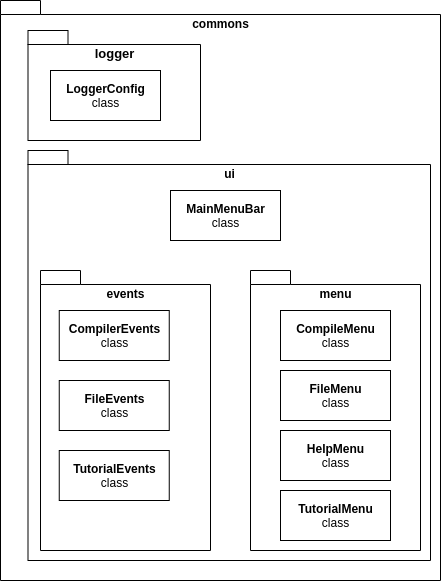
\includegraphics[width=0.8\linewidth]{img/CommonsPackage.png}
    \caption{Commons Package}
    \label{fig:conf}
\end{figure}

The classes are defined in two packages: 
\begin{itemize}
 \item \textbf{logger} package 
 
 This package contains only one class - \textbf{LoggerConfig}. This class defines the logging system used throughout the application. It is defined as a wrapper over the \textbf{Logger} class from Java Util, redirecting all the logs into a file called "app.log" and found in "<root\_folder>/output/logs" folder. The main operations wrapped are for logging information (\textit{infoLog}) and errors (\textit{errorLog}).
 
 
\item \textbf{ui} package

This package contains the user-defined graphical elements that are displayed in the views and the events that are triggered by Java swing elements. It is split in two subpackages:  
\begin{itemize}
	\item \textbf{menu} package
	
	This package contains the menu tabs that are displayed in the menu bar of the application. Each menu class contains a \textbf{JMenu} object and several \textbf{JMenuItem} objects, depending on the purpose of the menu. 
	\begin{enumerate}
	\item  \textbf{File Menu - FileMenu} 
	
	This menu is used for an user to access the file view. It holds a \textbf{New} tab for creating a new file, \textbf{Open} tab for opening an existing source code file, \textbf{Save} tab for saving the file that is displayed in the file view and \textbf{Exit} tab for exiting the application. 
	
	\item \textbf{Compile Menu - CompileMenu}
	
	This menu contains the tab \textbf{Compile File...} that, when pressed, it compiles the SueC source code when it is opened in the file view. 
	
	\item \textbf{Tutorial Menu - TutorialMenu}
	
	This menu contains the tabs that accesses the tutorial and guide views: \textbf{Tutorial List...} for tutorial view and \textbf{Help List...} for guide view, respectively.
	
	\item \textbf{Help Menu - HelpMenu}
	
	This menu contains only a tab called \textbf{About}. After pressing the tab, it opens a message dialog that displays information about the application.
	\end{enumerate}
	
	\item \textbf{events} package
	
	This package is represented by objects which contain the events that are triggered throughout the application. All the event classes act as a middleware between the view classes and the utility classes. Each event class represents a group of events specific to a menu or view.
	
	\begin{itemize}
		\item \textbf{File Events - FileEvents}
		
		This class encapsulates all the events triggered by the tabs in the \textbf{FileMenu}: creating a new file - \textit{newFileEvent}, opening an existing file - \textit{openFileEvent}, saving the file shown in the view - \textit{saveFileEvent}. Each event uses the operations from the \textbf{FileUtility} class. 
		
		\item \textbf{Compiler Events - CompilerEvents}
		
		This class contains the \textit{compileFileEvent} triggered when accessing the \textbf{Compile Menu} from the menu bar. The compile operation is called from the \textbf{CompilerUtility} class. 
		
		\item \textbf{Tutorial Events - TutorialEvents}
		
		This class contains the tutorial events that are triggered for the tutorial and guide views, respectively: loading the tutorials or guides from \textbf{TutorialUtility} object, and compiling a tutorial. When compiling a tutorial, operations from all the utility classes are used. A temporary file "temp.suc" is created in "<root\_folder>/resources/tempData" and the content of the code text area in the tutorial is saved in that file. After that, the file is compiled, then deleted. The output of the file is then sent back to the view to be checked if it is correct or not.
	\end{itemize}


Besides those, there are two graphical elements that are defined outside the packages:
\begin{itemize}
\item \textbf{Main Menu Bar - MainMenuBar}
	
	This class creates an instance of \textbf{JMenuBar}, the Java Swing object representation of a menu bar. It is used in the \textbf{BaseView} to define the menu bar where all the menu options are added and displayed on all views. 
	
\item \textbf{Text Area Element - TextAreaElement}

	This class extends the \textbf{JTextArea} Swing object, having specific requirements. It represents a text area that is read-only and supports word and line wrapping. I have used this object for creating the dynamic tutorial and guide views, respectively, for displaying more information in a readable matter - the title, description and task of a tutorial, and the title and description of a guide.
	
\end{itemize}
\end{itemize}
\end{itemize}

Besides the \textbf{logger} and \textbf{ui} packages, I have defined a class called \textbf{CommonElements}. It holds the common elements used on all views, having an instance of the menu bar and its menu items and specific fonts used for displaying the title, subtitle and info labels, respectively. Each font is bold and sans\_serif, but the difference between those is made via the size of it: title font - 36 pt, subtitle font - 20 pt, info font - 14 pt. 


\item \textbf{utilities} package

\begin{figure}[H]
    \centering
    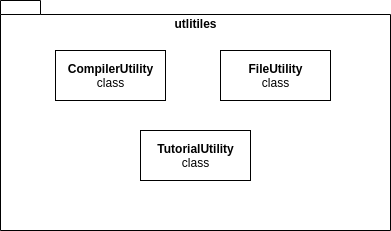
\includegraphics[width=0.8\linewidth]{img/UtilityPackage.png}
    \caption{Utility Package}
    \label{fig:conf}
\end{figure}

This package contains objects that define the utility operations. It wraps the actual low-level operations that are used in the application. Each class encapsulates a specific number of operations:
\begin{itemize}
\item \textbf{File Utility - FileUtility}
	
	The operations defined in this class are file handling operations. It is mainly triggered by the \textbf{FileEvents} class - creating, loading, saving and deleting a source code file given its path as the sole parameter (and the content of the file for saving the file), but also for running a tutorial - creating and deleting a temporary source code file.
\item \textbf{Tutorial Utility - TutorialUtility}

	This class is used for deserializing the JSON files "tutorials.json" and "guides.json" and loading the objects read into the tutorial and guide views, respectively.

\item \textbf{Compile Utility - CompileUtility}
	
	This class contains the actual operation of compiling the source code file. The steps for this method are: 
	\begin{enumerate}
	\item Running the compiler executable \textit{suec.out} stored in "<root\_folder>//resources//compiler" directory with the source code file's absolute path as the parameter of the executable.
	\item Reading the output of the compiler execution from "<root\_folder>//output//result//suec.output" file.
	\item Sending the output read to the view to be displayed.
	\end{enumerate}
\end{itemize}
\end{enumerate}

\section{Interpreter}

The other key component of this project is the interpreter. It is a simplified version of a compiler, having just a lexical and syntactic analysis without generating any machine code. This interpreter is an executable C program that interprets SueC source code files and returns the output accordingly.

This interpreter is comprised of four files:
\begin{enumerate}
\item Lexical analyzer - suec.l
\item Syntactic analyzer - suec.y
\item Tree parser - suec\_interpreter.c 
\item Commons header - suec\_header.h
\end{enumerate}


\begin{figure}[H]
    \centering
    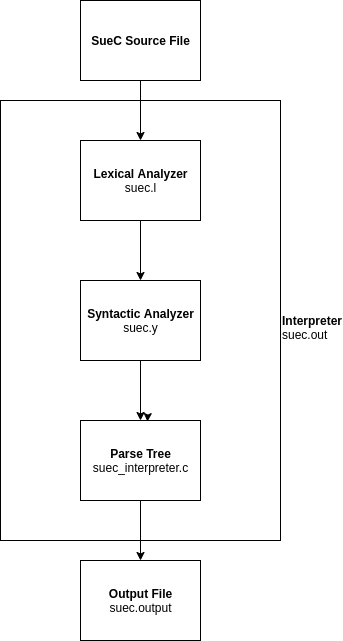
\includegraphics[width=0.6\linewidth]{img/InterpreterPipeline.png}
    \caption{Interpreter execution pipeline}
    \label{fig:conf}
\end{figure}

When interpreting a SueC Source code file, it follows an execution pipeline (see Figure 5.7). The source code is passed into the lexical analyzer in which each statement is split into tokens. These tokens are then passed to the syntactic analyzer, which associates them into a sentence based on their token. These sentences are interpreted using the tree parser, each sentence having a branch - one node is represented by a token. After the interpretation, the created tree is parsed in a bottom-up manner and the result of the parsing is then returned into an output file. 

\subsection{Lexical Analyzer - suec.l}

The lexical analyzer is the first part of the SueC interpreter. It is comprised of a single file called \textit{suec.l}, a lex file that is compiled using the UNIX GNU compiler with "lex -l suec.l" command in Terminal. This file is split into three zones, the border being marked with "\%\%":
\begin{enumerate}
	\item \textbf{Declarative zone}
	
	This zone is used for declaring global variables and including headers that are used in the file. These statements are encapsulated between these structures "\%\{" and "\%\}". In this case, the standard "stdlib.h", "stdio.h", "string.h" are included alongside "y.tab.h", generated after compiling the syntactic analyzer, and an external instance of \textit{yyin} that is used for instantiating the input file.
	
	\item \textbf{Tokenization zone}
	
	This zone contains all the regular expressions and rules that transform each part of a statement into a token. A statement is split into elements based on the patterns that are found in this zone and return a token associated to the pattern.
	These patterns are called regular expressions(abbreviated as regex) and are represented as:
	\begin{itemize}
		\item A specific string - used for declaring keywords of the programming language. They can be represented as a single word or a sentence with multiple words. In SueC's case, there are tokens declared for: \textit{int, string, if, else, for, while, read, write, length, copy, unite, compare} as keywords, and \textit{">=","<=","==","!="} as operations for comparing numbers (greater than equal, less than equal, equal and not equal, respectively).
		\item A rule - used for encapsulating raw data. These rules encapsulate characters that form an element of a variable length and are not mapped as a keyword or specific operation. This type is used for declaring variables, integers, strings and simple operations. 
		
		One rule is formed by placing a list of characters in a set defined by "["and "]". For an interval of ASCII characters, an "-" is used between two characters. This interval notation is added inside the square brackets. If just those delimiters are used, then any single occurence of a variable of that set has a token associated to it, as in the case of variable declaration or passing single operations. I have instantiated two tokens for defining variables represented by a single letter, each having the rule defined accordingly:
		
	\begin{itemize}
		\item "[A-Z]" for \textit{HCVAR} - variables defined by an uppercase letter
		\item "[a-z]" for \textit{LCVAR} - variables defined by a lowercase letter
		\item `[-()+*=/<>;"\}\{]` for returning simple operations - a token is not needed as the character is passed directly via \textit{yytext} which is a buffer that contains the string read for a pattern to be applied.
	\end{itemize}	
	
	An extension of the set rule is by adding a "+" after the set definition. This sign is used for reading strings of variable size with the characters in that set, accepting if the characters are repeated in the pattern. In this way, I have defined patterns for reading raw data:
	\begin{itemize}
		\item Integers - "[0-9]+".
		\item Strings - '"[a-zA-Z .,!?-]+"'
		\item Removing whitespaces - "[ \textbackslash t\textbackslash n]+"
	\end{itemize}
	\end{itemize}
	\item \textbf{Function zone}
	
	This zone is for declaring functions that are called during the tokenization when one pattern is found. In my case, I have used just to declare the \textit{yywrap()} function that is called internally when the interpreter starts working. 
\end{enumerate}

After the compilation of the said file, a lex C file called "lex.yy.c" is generated containing the patterns of the lex file as C functions that are called by the interpreter. 
\subsection{Syntactic Analyzer - suec.y}

The syntactic analyzer is the second part of the SueC interpreter. It is represented by a single file - \textit{suec.y}, a yacc file compiled using the UNIX GNU compiler with the following command: "yacc -y suec.y". Similar to the lexical anaylzer, the file is split into three zones with "\%\%" used as delimiters:

\begin{enumerate}
	\item \textbf{Declarative zone}
	
	This zone is used for declaring global variables and including headers that are used in the file. These statements are encapsulated between these structures "\%\{" and "\%\}". In this case, the standard "stdlib.h", "stdio.h", "string.h","stdarg.h" are included alongside "y.tab.h", generated after compiling the syntactic analyzer. Another header that is included is "suec\_header.h" that contains the definitions of the node structure of the tree parser - needed for creating the nodes inside the syntax zone. Beside the headers, in the delimiters are included the headers of the functions that are created in the function zone of the syntactic analyzer and the file variables for the output and log files, respectively. 
	
	Outside the delimiters, this zone also holds the declaration of the tokens that come from the lexical analyzer (which are terminals) and internal tokens (which are non-terminals). These tokens are, then, used in the syntax zone to define all the operations of the programming language. The tokens used for defining mathematical operations have also a property attached \textit{"\%left"} - for ensuring the left association that is used also in normal mathematics. 
	
	For receiving raw data alongside the tokens, the internal yylval is used as a buffer memory. This parameter is defined in the declarative zone of "suec.y" as a union of internal variables for storing different types of data. In my case, I have defined an union consisting of:
	\begin{itemize}
		\item An integer - \textit{iValue} - used for storing integers under \textit{NUM} token.
		\item A character - \textit{variable} - used for storing the variable code under \textit{HCVAR} and \textit{LCVAR} tokens, respectively.
		\item A character pointer - \textit{word} - used for storing string under \textit{WORD} token.
		\item A node operand - \textit{np} - used for storing the non-terminal operands.
	\end{itemize}
	
	\item \textbf{Syntax zone}
	
	This zone contains all the definitions of the operations that the programming language can perform. These operations are defined as patterns based on the tokens declared before, creating different "sentences" that have an operation associated. Each non-terminal defined can have multiple cases of return, as each pattern of the non-terminal is separated by an "|" representing an "or" between those patterns. In the case for "suec.y", I have grouped the statements into a tree pattern based on their functionality type:
	\begin{itemize}
	\item \textit{Conditional Statement}
	
	Conditional statements are statements that check a condition performed in a statement and performs accordingly to the outcome of the said test. In general, it is represented by "if" statements. In SueC, I have created two rules that represent the if statement as in C programming language: \textit{IF '(' expression ')' statement} and \textit{IF '(' expression ')' statement ELSE statement} (for if-then-else). These statements are encapsulated under the non-terminal \textit{condStatement}
	
	\item \textit{Loop Statement}
	
	Loop statements are statements that perform operations under a timed interval defined by the condition(s) defined in the statement. It can be a fixed interval ("for" loop) or an variable interval ("while" loop). I have implemented both "for" and "while" loops, keeping the structure from C:
	\begin{itemize}
	\item \textit{FOR '(' simplestatement ';' expression ';' expression ')' statement} - "for" statement as \textit{forStatement}
	\item \textit{WHILE '(' expression ')' statement} - "while" statement as  \textit{whileStatement}
	\end{itemize}
	Both non-terminals are encapsulated under the \textit{loopStatement} non-terminal.
	\item \textit{Simple Statement}
	
	A simple statement is a represented by a simple operation that does not require any conditions or creating loops. These type of statements are used for creating the other types (conditional or loop). One major difference between this and the other types is that it has an end character - a semicolon for showing that statement is ended. I have grouped these statements under the \textit{simplestatement} non-terminal also based on their functionality: 
	\begin{itemize}
		\item \textit{variableStatement} non-terminal
		
		This non-terminal encapsulates the declaration statements that can be performed in SueC. These patterns hold the same structure: <Data\_Type> <Variable\_Type> and are defined directly using any permutation of the values, shown in the Table 5.1.
		\begin{table}[H]
\centering


\begin{tabular}{cclll}
\cline{1-2}
\multicolumn{1}{|c|}{\textless{}Data\_Type\textgreater{}} & \multicolumn{1}{c|}{\textless{}Variable\_Type\textgreater{}} &  &  &  \\ \cline{1-2}
\multicolumn{1}{|c|}{INTEGER}                             & \multicolumn{1}{c|}{HCVAR}                                   &  &  &  \\ \cline{1-2}
\multicolumn{1}{|c|}{STRING}                              & \multicolumn{1}{c|}{LCVAR}                                   &  &  &  \\ \cline{1-2}
\multicolumn{1}{l}{}                                      & \multicolumn{1}{l}{}                                         &  &  & 
\end{tabular}

\caption{Variable Statement Table}
\end{table}

	\item Input/output expressions
	
	These expressions are defined directly, without any other encapsulated non-terminals. In this case, the input/output statements are defined accordingly:
	\begin{itemize}
	\item Input statement - \textit{"READ variable"}
	\item Output statement - \textit{"WRITE expression"}
	\end{itemize} 
	
	\item Assignment expression - operation exclusively for integer variables: \textit{"variable '=' expression}
	
	\item \textit{expression} non-terminal
	
	This non-terminal is the base element that is used throughout all the statements, as it holds the simple operations. Most of the patterns are with the structure \textit{expression <op> expression}, where <op> can be one of the values from Table 5.2 .
	
\begin{table}[H]
\centering

\label{tab:my-table}
\begin{tabular}{|c|l|l|ll}
\cline{1-3}
Mathematical           & \multicolumn{1}{c|}{String} & Conditional                   &  &  \\ \cline{1-3}
+                      & \multicolumn{1}{c|}{COPY}   & \textless{}                   &  &  \\ \cline{1-3}
-                      & \multicolumn{1}{c|}{UNITE}  & \textgreater{}                &  &  \\ \cline{1-3}
*                      & COMPARE                     & \textit{\textless{}= - LE}    &  &  \\ \cline{1-3}
/                      &                             & \textit{\textgreater{}= - GE} &  &  \\ \cline{1-3}
\multicolumn{1}{|l|}{} &                             & \textit{!= - NE}              &  &  \\ \cline{1-3}
\multicolumn{1}{|l|}{} &                             & \textit{== - EQ}              &  &  \\ \cline{1-3}
\end{tabular}

\caption{Available values for \textless{}op\textgreater{}}
\end{table}

The \textit{LENGTH expression} is defined without the left \textit{expression} variable as it only used for one string. Besides the operation patterns, the data terminals are used directly here as standalone cases for returning raw data: \textit{NUM} for integers, \textit{WORD} for strings, \textit{variable} for variable characters (\textit{HCVAR} and \textit{LCVAR}).
	\end{itemize}
	\end{itemize}
	
	All these sentences are then preceded by curly brackets that contain what operations need to be done in case of one sentence. In SueC's case, at the start of sentences, the \textit{execute\_node} from the interpreter is called for executing the statement (at \textit{program: program statement} - the start pattern of the application) and the rest of the statements where also terminals are present contain call functions for creating the specific node types that can be parsed and interpreted. These functions are defined in the function zone.
	
	\item \textbf{Function zone}
	
	This zone is used for creating functions that have their headers defined in the declaration zone. Besides the \textit{main(int argc, char **argv)} function which contains the call to parse the tokens and opens the log and output files to be written accordingly, I have defined functions for creating tree nodes according to their type:
	\begin{itemize}
		\item \textit{constType} 
		
		This is associated to nodes that hold raw constant data and their associated functions are: \textit{leafInt()} and \textit{leafString()}.
		
		\item \textit{idType}
		
		This is associated to nodes that hold the variable information - in order to access the stored data. The associated function is: \textit{iden()}
	
		\item \textit{operType}
		
		This is associated to nodes that hold actual operation values and parameters. The function is: \textit{operand()}
	\end{itemize}
\end{enumerate}
 
\subsection{Tree Parser}

The tree parser is the last part of the SueC interpreter. The aim of this component is to parse the trees that are generated by each statement that has passed the syntactic analysis. I have implemented the tree parsing inside another file called "suec\_interpreter.c". Beside this, I have used a header file "suec\_header.h" that is included also in the syntactic analyzer.

The header file contains the tree node structure definitions, which are encapsulated inside another node definition. The node structure type is called \textit{nodeType} and contains:
\begin{itemize}
	\item A \textit{nodeEnum} type variable. This enum value is defined in this header file and contains: \textit{constType} for constants, \textit{idType} for identifiers (variables) and \textit{operType} for operands. It is used to differentiate what node is read/written when parsing/creating. 
	\item A union that contains the actual data of the nodes, each node being specific to the type defined in the \textit{nodeEnum}: \textit{constNodeType constant} for constant node, \textit{idNodeType id} for identifier node and \textit{operNodeType oper} for operation node.  
\end{itemize}

Each node type from the enum has its own structure defined in separate struct values:
\begin{itemize}
	\item \textbf{constNodeType}
	
	This node type defines nodes specific for constant values, both integers and strings. This structure contains: an integer called \textit{type} for holding the token that is either an integer or string, an integer \textit{iValue} as the buffer for integers and a string(char*) \textit{sValue} as the buffer for strings.
	
	\item \textbf{idNodeType}
	
	This node type defines nodes specific for identifiers (variables). Structurally, it contains three integers: \textit{valueType} which holds the data type of the variable (\textit{INTEGER} or \textit{STRING}), \textit{charType} which holds the type of the variable character - either uppercase letter \textit{HCVAR} or lowercase letter \textit{LCVAR} - and \textit{value} which holds the character value between 0 and 25 - used when accessing the buffer data. The \textit{value} is represented accordingly to the \textit{charType}: the actual variable stored has the ASCII code equal to the addtion of \textit{value} and the ASCII code of 'a'(for \textit{LCVAR}) or 'A'(for \textit{HCVAR}).
	
	\item \textbf{operNodeType}
	
	This node type defines nodes specific for operations that are performed: from simple mathematical operations to conditional or loop statements. It contains a value \textit{oper} for storing what operation is done - the token of of the operation, \textit{nops} for storing the number of operands and \textit{op} - a dynamic list of \textbf{nodeType} nodes that contain the actual operands of the operation.
\end{itemize}

Other than the tree node structure, there is a declaration of the buffer memory which holds the actual data of the varaibles. There are two arrays, one for uppercase variables called \textit{hcSymbols} and the other for lowercase variables called \textit{lcSymbols} which have as key the \textit{value} from the \textbf{idNodeType} node. The value of these buffers are also a structure defined as \textbf{symVar} which holds: an integer \textit{valueType} that holds the value of what type of data is used - instantiated with the value of the same name in \textbf{idNodeType} and an union that consists of an integer buffer \textit{iValue} and a string buffer \textit{sValue}.

The tree parser is a C file that contains the definitions of the functions that executes the parsing of the nodes. Each function defined has only one paramater in the function header - a pointer to the \textit{nodeType}. The syntactic analyzer calls only one function - \textit{execute\_node()} - which in return gives the of the node. This function calls a different function based on the \textit{type} value of the node given as parameter:

\begin{itemize}
	\item \textit{execute\_const()} for \textit{constType}
	
	This function parses the \textit{constNodeType} nodes, returning the value based on the type: the integer \textit{iValue} for integers or the string \textit{sValue} for strings. 
	
	\item \textit{execute\_id()} for \textit{idType}
	
	This function parses the \textit{idNodeType} nodes, returning the value from the buffer memory \textit{hcSymbols} or \textit{lcSymbols}. For choosing what value to return, a switch is used to redirect to other functions based on the data type returned: \textit{execute\_id\_int()} for integers and \textit{execute\_id\_str()} for strings. Each of these functions return the value based on the \textit{charType} (\textit{HCVAR} or \textit{LCVAR}), returning the value from the buffer using the \textit{value} of the \textit{idNodeType} as the key of the buffer memory. 
	
	\item \textit{execute\_oper()} for \textit{operType}
	
	This functions parses the \textit{operNodeType} nodes, returning the value after performing the operations. Basically, this function calls recursively the \textit{execute\_node()} function in order to obtain the result. The end of the recursions are the other functions: \textit{execute\_const()} and \textit{execute\_id()}. Each operation is parsed accordingly, choosing the operation according to the value of \textit{oper} parameter in the node. After seeing the operation, the \textit{op} list is traversed and each node is parsed in the pattern of the operation that is performed, the pattern being kept as from the syntactic analyzer.  
\end{itemize}


\section{SueC Programming Language}

SueC programming language is the key programming language of this project, being implemented with the help of the interpreter. It is an imperative programming language, having simple structures similar to C and Python programming languages. The aim of this SueC is to be closer to the pseudocode and to be easily understood and learnt by people with little to no experience in programming.

\subsection{Syntax}

\subsubsection{Keywords}
	The main keywords used in SueC are listed in the Table 5.3.
	
\begin{table}[H]
\centering
\begin{tabular}{|c|c|p{8cm}|}
\hline
\textit{\textbf{Keyword}} & \textit{\textbf{Example}}                                                                                                                                                 & \multicolumn{1}{c|}{\textit{\textbf{Observation}}}                                                                                                                                                                                                                                                                                     \\ \hline
\textbf{int}              & int \textless{}var\textgreater{};                                                                                                                                         & Used for defining an integer variable.                                                                                                                                                                                                                                                                                                 \\ \hline
\textbf{string}           & string \textless{}str\_var\textgreater{};                                                                                                                                 & Used for defining a string variable.                                                                                                                                                                                                                                                                                                   \\ \hline
\textbf{if}               & \begin{tabular}[c]{@{}c@{}}if (\textless{}cond\textgreater{}) \\ \textless{}stmt\textgreater{}\end{tabular}                                                               & Used for defining a conditional statement. Can be defined without the use of "else" keyword.                                                                                                                                                                                                                                           \\ \hline
\textbf{else}             & \begin{tabular}[c]{@{}c@{}}if (\textless{}cond\textgreater{}) \\     \textless{}stmt\textgreater{};\\ else             \\     \textless{}stmt\textgreater{};\end{tabular} & Used for defining a conditional statement alongside "if" keyword when the condition defined is not fulfilled and other statements need to be done.                                                                                                                                                                                     \\ \hline
\textbf{for}              & \begin{tabular}[c]{@{}c@{}}for (\textless{}stmt\textgreater{};\textless{}cond\textgreater{};\textless{}stmt\textgreater{})\\ \textless{}stmt\textgreater{};\end{tabular}  & Used for defining a loop statement having a fixed interval defined by three statements.                                                                                                                                                                                                                                                \\ \hline
\textbf{while}            & \begin{tabular}[c]{@{}c@{}}while(\textless{}cond\textgreater{})\\ \textless{}stmt\textgreater{};\end{tabular}                                                             & Used for defining a loop statement having a variable interval - with only one conditional expression.                                                                                                                                                                                                                                  \\ \hline
\textbf{read}             & read \textless{}var\textgreater{};                                                                                                                                        & Used for input operation. It reads data from the user and stores it in a variable.                                                                                                                                                                                                                                                     \\ \hline
\textbf{write}            & write \textless{}stmt\textgreater{};                                                                                                                                      & Used for output operation. It displays the data to the user: integer or strings directly as constants or as the result of simple operations.                                                                                                                                                                                           \\ \hline
\textbf{length}           & length \textless{}str\_var\textgreater{};                                                                                                                                 & Used for returning the length of a string - given as a constant or a string variable.                                                                                                                                                                                                                                                  \\ \hline
\textbf{copy}             & \textless{}dest\_str\textgreater copy \textless{}src\_str\textgreater{};                                                                                                  & Used for copying the source string into the destination string. The source can be a constant string or a string variable. The destination string is a string variable. The result is stored in the destination string.                                                                                                                 \\ \hline
\textbf{unite}            & \textless{}dest\_str\textgreater unite \textless{}src\_str\textgreater{};                                                                                                 & Used for unifying the source string with the destination string. The source can be a constant string or a string variable. The destination string is a string variable. The result is stored in the destination string.                                                                                                                \\ \hline
\textbf{compare}          & \textless{}str\_1\textgreater compare \textless{}str\_2\textgreater{};                                                                                                      & Used for comparing the source string with the destination string. Both strings can be either constants or string variables. The result returned is an integer variable that displays which string has a greater value: a negative number for the second string, a positive number for the first string and 0 if the strings are equal. \\ \hline
\end{tabular}
\caption{Syntax table}
\label{tab:my-table}
\end{table}

\subsubsection{Identifiers}

Identifiers are the name of the variables that are used in SueC source code. The identifiers are defined as simple letters from the English alphabet, both uppercase and lowercase, thus having 52 different variables. These are used when storing data in memory and accessing it for different operations that are supported in this programming language.

\subsubsection{Data Types}

In SueC programming language, there are two main data types that are defined and used:

\begin{enumerate}
 	\item \textbf{Integers}
 	
 	Integers are numbers that are displayed in decimal base and are used in simple mathematical operations and comparisons. These can be used directly as constants written normally or stored in variables that have been defined as "int <var>".
 	 
 	\item \textbf{Strings}
 	
 	Strings are words that contain letters from the alphabet, numbers, spaces and punctuation symbols. It holds the same syntax as specified in C and Python - the strings are defined between two quotation marks (""). After defining a string variable, it automatically holds a null value '\textbackslash 0' in memory, that is not displayed on screen, to ensure the end of the string. 
\end{enumerate}

\subsubsection{Operations}

	In this programming language, there are operations defined specifically just for the data types implemented. These operations are all binary operations that return an output directly or store it in one of the parameters. These are:
	\begin{itemize}
		\item \textit{Integer operations}
		
		These operations are simple mathematical operations that are applied using constants and integer variables. These operations are grouped as mathematical and comparison operations. The syntax of these operations are displayed in the tables below (see tables 5.4 and 5.5).


\begin{table}[H]
\centering
\resizebox{\textwidth}{!}{%
\begin{tabular}{|c|c|p{8cm}|}
\hline
\textit{\textbf{Operation}}  & \textit{\textbf{Syntax}}                                      & \multicolumn{1}{c|}{\textit{\textbf{Explanation}}}                                                                                                                                 \\ \hline
\textbf{'+'(additon)}        & \textless{}el\_1\textgreater + \textless{}el\_2\textgreater{} & Returns the additon of \textless{}el\_1\textgreater and \textless{}el\_2\textgreater{}.                                                                                            \\ \hline
\textbf{'-'(subtraction)}    & \textless{}el\_1\textgreater - \textless{}el\_2\textgreater{} & Returns the subtraction of \textless{}el\_2\textgreater from \textless{}el\_1\textgreater{}.                                                                                       \\ \hline
\textbf{'*'(multiplication)} & \textless{}el\_1\textgreater * \textless{}el\_2\textgreater{} & Returns the multiplication of \textless{}el\_1\textgreater and \textless{}el\_2\textgreater{}.                                                                                     \\ \hline
\textbf{'/'(division)}       & \textless{}el\_1\textgreater / \textless{}el\_2\textgreater{} & Returns the division of \textless{}el\_1\textgreater by \textless{}el\_2\textgreater{}.                                                                                            \\ \hline
\textbf{'='(assignment)}     & \textless{}var\textgreater = \textless{}elem\textgreater{}    & It assigns the value of \textless{}elem\textgreater to the variable \textless{}var\textgreater{}; \textless{}elem\textgreater can also be one of those above mentioned operations. \\ \hline
\end{tabular}%
}
\caption{Mathematical operations}
\label{tab:my-table}
\end{table}

For comparison operations, the output returned is 1 if the statement is true and 0 otherwise. These operations are used in conditional statements, mainly.

% Please add the following required packages to your document preamble:
% \usepackage{graphicx}
\begin{table}[H]
\centering
\resizebox{\textwidth}{!}{%
\begin{tabular}{|c|c|p{8cm}|}
\hline
\textit{\textbf{Operation}}  & \textit{\textbf{Syntax}}                                      & \multicolumn{1}{c|}{\textit{\textbf{Explanation}}}                                                                                                                                 \\ \hline
\textbf{'+'(additon)}        & \textless{}el\_1\textgreater + \textless{}el\_2\textgreater{} & Returns the additon of \textless{}el\_1\textgreater and \textless{}el\_2\textgreater{}.                                                                                            \\ \hline
\textbf{'-'(subtraction)}    & \textless{}el\_1\textgreater - \textless{}el\_2\textgreater{} & Returns the subtraction of \textless{}el\_2\textgreater from \textless{}el\_1\textgreater{}.                                                                                       \\ \hline
\textbf{'*'(multiplication)} & \textless{}el\_1\textgreater * \textless{}el\_2\textgreater{} & Returns the multiplication of \textless{}el\_1\textgreater and \textless{}el\_2\textgreater{}.                                                                                     \\ \hline
\textbf{'/'(division)}       & \textless{}el\_1\textgreater / \textless{}el\_2\textgreater{} & Returns the division of \textless{}el\_1\textgreater by \textless{}el\_2\textgreater{}.                                                                                            \\ \hline
\textbf{'='(assignment)}     & \textless{}var\textgreater = \textless{}elem\textgreater{}    & It assigns the value of \textless{}elem\textgreater to the variable \textless{}var\textgreater{}; \textless{}elem\textgreater can also be one of those above mentioned operations. \\ \hline
\end{tabular}%
}
\caption{Comparison operations}
\label{tab:my-table}
\end{table} 

\item \textit{String operations}

These operations use strings or string variables as input elements. These operations return strings or integers.
\begin{table}[H]
\centering
\resizebox{\textwidth}{!}{%
\begin{tabular}{|c|c|p{8cm}|}
\hline
\textit{\textbf{Operation}} & \textit{\textbf{Syntax}} & \multicolumn{1}{c|}{\textit{\textbf{Explanation}}} \\ \hline
\textbf{length}           & length \textless{}str\_var\textgreater{};                                                                                                                                 & Used for returning the length of a string - given as a constant or a string variable. The value returned is an integer.                                                                                                                                                                                                                                                  \\ \hline
\textbf{copy}             & \textless{}dest\_str\textgreater copy \textless{}src\_str\textgreater{};                                                                                                  & Used for copying the source string into the destination string. The source can be a constant string or a string variable. The destination string is a string variable. The result is stored in the destination string.                                                                                                                 \\ \hline
\textbf{unite}            & \textless{}dest\_str\textgreater unite \textless{}src\_str\textgreater{};                                                                                                 & Used for unifying the source string with the destination string. The source can be a constant string or a string variable. The destination string is a string variable. The result is stored in the destination string.                                                                                                                \\ \hline
\textbf{compare}          & \textless{}str\_1\textgreater compare \textless{}str\_2\textgreater{};                                                                                                      & Used for comparing the source string with the destination string. Both strings can be either constants or string variables. The result returned is an integer variable that displays which string has a greater value: a negative number for the second string, a positive number for the first string and 0 if the strings are equal. \\ \hline
\end{tabular}%
}
\caption{String operations}
\label{tab:my-table}
\end{table}
	\end{itemize}
\section{Use Cases}
 For this project, there are few use cases that are available (see Figure 5.8). An user can:
 \begin{itemize}
 \item Create a SueC source code file.
 \item Open a SueC source code file.
 \item Edit a SueC source code file.
 \item Compile a SueC source code file.
 \item Perform a tutorial of the application.
 \item Read a guide that is attached to the application.
 \end{itemize}
 
\begin{figure}[H]
    \centering
    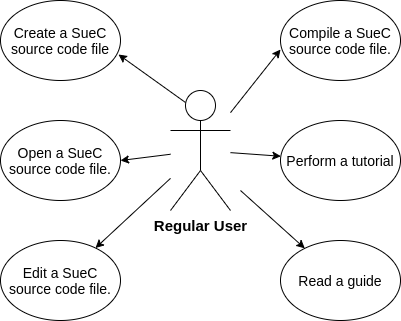
\includegraphics[width=0.6\linewidth]{img/UseCaseDiag.png}
    \caption{Use Case Diagram}
    \label{fig:conf}
\end{figure}

There is only one type of user: a regular person that can be anyone who has little to no experience in programming and wants to learn about computer programming basics. 

\subsection{Use Case Specification - Performing a tutorial}

\subsubsection{Brief Description}

The purpose of this specification is to capture the flow of events that an actor must follow in order to perform a tutorial. The primary actor is a regular user that can be any person with little to no experience in computer programming. 

\subsubsection{Preconditions}

The actor has the application open at tutorials list tab. 

\subsubsection{Postconditions}

The tutorial is finished and the actor proceeds to another tutorial or returns to the tutorial list menu when finishing the last tutorial.

\subsubsection{Flow of Events}

The flow of events are displayed in Figure 5.9. There is a basic flow that ensures a simple functionality of the feature, but there are also some alternative flows that can be triggered in some cases.

\begin{figure}[H]
    \centering
    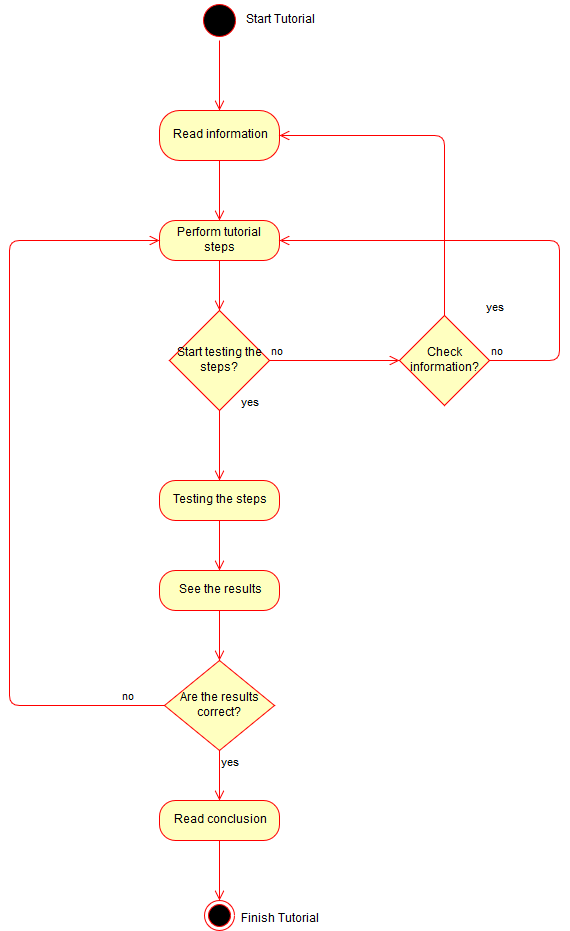
\includegraphics[width=0.5\linewidth]{img/UCTutorial.png}
    \caption{Flow of events for performing a tutorial}
    \label{fig:conf}
\end{figure}

\begin{itemize}
	\item \textbf{Basic Flow}
	This use case starts when the actor wants to perform a tutorial selected from the tutorial list menu.
	
	Flow steps:
	\begin{enumerate}
		\item The actor reads the brief information about the concept and the steps to be performed.
		\item The actor performs the steps explained before.
		\item The actor checks the code written after step 2.
		\item The system tests the code written by the actor.
		\item The system returns and displays the results from the test.
		\item The system decides that the results returned are correct and display the "Next/Finish" button.
		\item The actor presses the button displayed after step 6 and finishes the tutorial.
	\end{enumerate}
	
	This use case ends after step 7 and a the following tutorial from the tutorial list is displayed or returns to the main tutorial list menu of the application.
	\item \textbf{Alternative Flows}
	
	These alternative flows are occured in these cases:
	
	\begin{itemize}
		\item The actor did not check the code and wants to read the description area. In this case, the user will return to step 1.
		\item The actor did not check the code and does not want to read the information text. In this case, the user will read the steps written in the task area.
		\item The system returns wrong results. In this case, the system will display the results alongside with a message "Wrong! Do it again!" and returns to step 2 in order to let the actor perform changes on the code.
		\item At any time, the tutorial can be aborted by opening or creating a new SueC source code file, redirecting to the \textit{File View} or accessing the tutorial list menu. In both cases, the tutorial is reset.
	\end{itemize}
\end{itemize}


\section{Example of Execution - Compiling a file}
One of the main operations that the application supports is to compile a SueC source code file. This is done from the editor application, shown in Figure 5.10.
\begin{figure}[H]
    \centering
    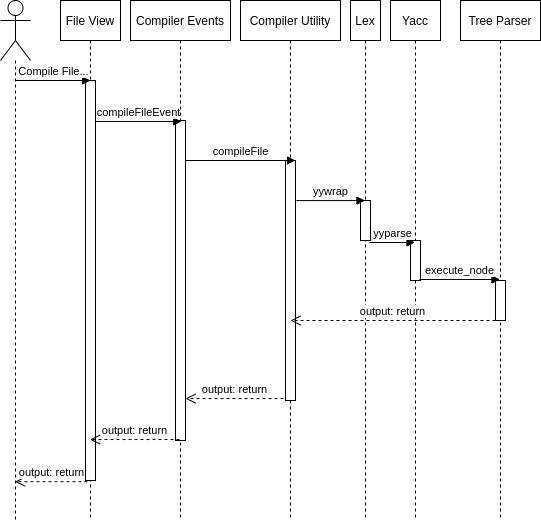
\includegraphics[width=0.52\linewidth]{img/SeqDiag.png}
    \caption{Sequential Diagram}
    \label{fig:conf}
\end{figure}

For a source file to be compiled, the following sequence of operations are done:

\begin{enumerate}
\item After the user finishes editing the source code file while in the file view, he presses the "Compile file..." tab from the "Compile" menu, triggering the tab event.

\item The file is automatically saved and the \textit{compileFileEvent} from the Compiler Events class is triggered, having the file path as parameter.

\item The \textit{compileFileEvent} method calls the \textit{compileFile} method from the Compiler Utility class, passing the file path as parameter.

\item The \textit{compileFile} method starts the process of running the compiler having the parameter the file path of the source code file.

\item The compiler receives the file path and starts parsing the file by tokenizing the statements from the file, action done using the Lex file. The tokens are sent to the Yacc file. 

\item The tokens are read by the Yacc file and tree are formed. Each statement from the source code have an associated tree, having the number of nodes equal to the number of tokens.

\item After the tree nodes are formed, they are parsed by the tree parser and the result obtained is written in the output file. 

\item The compiler has finished running and read the output from the compiler output file.

\item The content of the output file is returned by \textit{compileFile} to the \textit{compilerFileEvent} method.

\item The result returned to \textit{compileFileEvent} is returned to the File View and displayed in the result text area for the user to check.
\end{enumerate}


\chapter{Testing and Validation}

\section{Testing}

I have tested the application manually, using principles similar to the manual testing that is currently used in companies nowadays. Mainly, I have tested the functionalities in a simple manner for checking if there are some defects and bugs found during the development of the project. After these fixes, I have tested the response time of the application in two situations:

\begin{itemize}

\item \textit{Compiling a file}

 For compiling a file, I have tested the response time from the point the user presses the "Compile File..." tab to the system returning the result from the compiler. Despite running the code for several times, the response time remained constant at 0.5 seconds.

\item \textit{Running a tutorial}

 For running a tutorial, I have tested the response time from the point the user presses the "Compile Tutorial" button in the tutorial page until the system returns the output. As the tutorial list was already loaded in the cache memory of the application, the load of the tutorial in the view was instant. The response time remained constant as for compiling the file, in 0.5 seconds, in either case: getting a wrong result and a successful result. After getting the result, in the same time the button for getting to the next tutorial/finishing all the tutorials is activated instantly.
\end{itemize}
\section{Validation}

For validation, I have implemented a logging system for monitoring the activity of the components and their objects. This system is implemented in a simple manner to be supported in the editor applicator and the SueC interpreter. Each component of the application has its own log file: \textit{app.log} for the editor application and \textit{suec.log} for the interpreter. Both files are found under the same folder: "<root\_project>/output/logs/" and can be accesed by a regular user easily, as they can be read from any text editor files. 

\subsection{Interpreter Logging System}

On the interpreter side, the logging system is pretty simple, being a reusage of \textit{fprintf} function that is integrated in C programming language. At the start of the compiler life cycle, a \textit{FILE} variable pointer that accesses the log file "<root\_project>/output/logs/suec.log" with writing rights. This pointer is used to show where to log the activities of the syntactic analyzer and tree parser. Each log in the interpreter contains two elements:
\begin{itemize}
	\item A tag put between "[" and "]" - it can be either "[Yacc]" for the syntactic analyzer or "[Interpreter]" for the tree parser.
	\item The actual message, being "Got in <token>", where <token> is represented by any of the tokens of the lexical analyzer. 
\end{itemize} 

In the case of the tokens that represent the raw data(NUM, VALUE or WORD), their value is also logged in order to ensure the correctness of data that is parsed.


\subsection{Editor Logging System}

The editor logging system is a bit more complex than the one used in the interpreter, as it is specific to the Java applications. This system is designed as a wrapper over the existing \textit{java.util.logging.Logger} class - called \textit{LoggerConfig} and defined under the \textit{commons} package. This class is initialized at the start of the application life cycle, opening the log file  "<root\_project>/output/logs/app.log". The other objects call the static methods \textit{infoLog} and \textit{errorLog} accordingly to their needs. Each log written by this system contains:
\begin{itemize}
\item A log level that is defined internally in the wrapped methods: \textit{LogLevel.Info} for \textit{infoLog} and \textit{LogLevel.Severe} for \textit{errorLog}, respectively .
\item A message  that is displayed on the screen. This message is defined by a tag and a description. The tag is a string defined in each object the logger to show the source of the log call. The description contains information about the method that is called inside that object. 
\item Optionally, parameters. The parameters are sent as an \textit{java.lang.Object} array to the logging system and are displayed based on their position in the list and their identifier position in the description string. An identifier in the string is defined as "\{id\}", where id can be an index number from 0 to the size of the object array. 
\end{itemize}
\chapter{User's manual}

\section{Prerequesities}

\subsection{Hardware resources}

As hardware resources, the minimal system requirements are similar to running Ubuntu version 18.04:
\begin{itemize}
\item A dual-core processor with a clock speed of 2 GHz
\item 4 GB RAM
\end{itemize}

\subsection{Software resources}

The software resources needed for running the project are:
\begin{itemize}
	\item A Linux operating system - recommended: Ubuntu starting with the 18.04 version
	\item Java JDK - OpenJDK version 11. 
	\item flex and bison for the interpreter
\end{itemize}
\section{Step-by-step Guide}

\chapter{Conclusions}

About. 5\% of the whole

Here your write:
\begin{itemize}
\item a summary of your contributions/achievements,
\item a critical analysis of the achieved results,
\item a description of the possibilities of improving/further development.
\end{itemize}
\section{Title}
\section{Other title}


%\addcontentsline {toc}{chapter}{Bibliography} 
\bibliographystyle{IEEEtran} 
\bibliography{thesis}%same file name as for .bib

\appendix
\chapter{Relevant code}

\begin{verbatim}
 /** Maps are easy to use in Scala. */
object Maps {
  val colors = Map("red" -> 0xFF0000,
                   "turquoise" -> 0x00FFFF,
                   "black" -> 0x000000,
                   "orange" -> 0xFF8040,
                   "brown" -> 0x804000)
  def main(args: Array[String]) {
    for (name <- args) println(
      colors.get(name) match {
        case Some(code) =>
          name + " has code: " + code
        case None =>
          "Unknown color: " + name
      }
    )
  }
}
\end{verbatim}

\chapter{Other relevant information (demonstrations, etc.)}


\chapter{Published papers}

\end{document}
